In this section, we introduce the main concept and hypothesis of the paper. % from a psycholinguistic perspective. 
We provide a technical definition of the memory--surprisal tradeoff curve, and we prove a theorem showing that more efficient memory--surprisal tradeoffs are possible in languages exhibiting information locality, i.e., in languages where words that depend on each other are close to each other. This theorem establishes the formal link between memory efficiency in online processing and locality in word order.

The memory--surprisal tradeoff applies in both language production and comprehension---more generally, it applies to any system that incrementally produces sequences or extracts information from them. Below, we will develop the theory first in terms of language comprehension; we return to the production perspective in the General Discussion. % (Section~\ref{sec:discussion}).



\subsection{An information-theoretic model of online language comprehension}
\label{sec:listener-tradeoff}

We begin developing our model by considering the process of language comprehension, where a listener is processing a stream of words uttered by an interlocutor.
Experimental research has established three properties of online language comprehension: (1) listeners maintain some information about the words received so far in incremental memory, (2) listeners form probabilistic expectations about the upcoming words \citep[e.g.][]{altmann1999incremental,staub2006syntactic,kuperberg2016we}, and (3) words are easy to process to the extent that they are predictable based on a listener's memory of words received so far \citep{hale2001probabilistic,levy2008expectation,futrell2020lossy}. 
See General Discussion % (Section~\ref{sec:discussion})
for discussion of how our model is related to theories that do not explicitly make these assumptions.

We formalize these three observations into postulates intended to provide a simplified picture of what is known about online language comprehension. Consider a listener comprehending a sequence of words $w_1, \dots, w_t, \dots, w_n$, at an arbitrary time $t$.
\begin{enumerate}
    \item Comprehension Postulate 1 (Incremental memory). At time $t$, the listener has an incremental \key{memory state} $m_t$ that contains her stored information about previous words. The memory state is characterized by a \key{memory encoding function} $M$ such that $m_t = M(w_{t-1}, m_{t-1})$.
    \item Comprehension Postulate 2 (Incremental prediction). The listener has a subjective probability distribution at time $t$ over the next word $w_t$ as a function of the memory state $m_t$. This probability distribution is denoted $P(w_t|m_t)$.
    \item Comprehension Postulate 3 (Linking hypothesis). Processing a word $w_t$ incurs difficulty proportional to the \key{surprisal} of $w_t$ given the memory state $m_t$:
    \begin{equation}
    \label{eq:lossy-surp}
    \text{Difficulty} \propto -\log P(w_t | m_t).
\end{equation}
\end{enumerate}
The claim that processing difficulty should be directly proportional to surprisal comes from \key{surprisal theory} \citep{hale2001probabilistic,levy2008expectation}, an established psycholinguistic theory that can capture reading time effects related to garden-path disambiguation, antilocality effects, and effects of syntactic construction frequency. Surprisal is a robust linear predictor of reading times in large-scale eye-tracking studies based on naturalistic text \citep{smith2013effect,goodkind-predictive-2018,aurnhammer2019evaluating,wilcox2020predictive}, and effects of surprisal have been observed for units as small as phonemes \citep{gwilliams2020neural}. There are several converging theoretical arguments for surprisal as a measure of processing cost \citep{levy2008expectation,smith2013effect}.
Surprisal theory is compatible with different views on the mechanisms underlying prediction, and can reflect different mechanisms such as preactivation and integration~\citep{kuperberg2016we}.
We do not assume that listeners explicitly compute a full-fledged distribution $P(w_t|m_t)$; we view $P(w_t|m_t)$ as a formalization of the probabilistic expectations that listeners form during comprehension.

%@inproceedings{wilcox2020predictive,
%author={Ethan G. Wilcox and Jon Gauthier and Jennifer Hu and Peng Qian and Roger P. Levy},
%title={On the predictive power of neural language models for human real-time comprehension behavior},
%year={2020},
%booktitle={Proceedings of CogSci 2020},
%pages={1707--1713}}

%@article{aurnhammer2019evaluating,
%author={Christoph Aurnhammer and Stefan L. Frank},
%title={Evaluating information-theoretic measures of word prediction in naturalistic sentence reading},
%journal={Neuropsychologia},
%volume={134},
%year={2019},
%pages={107198}}


Our expression~(\ref{eq:lossy-surp}) differs from the usual formulation of surprisal theory in that we consider predictability based on a (potentially lossy or noisy) memory representation $m_t$, rather than predictability based on the true complete context $w_1, \dots, w_{t-1}$. The generalization to lossy memory representations is necessary to capture empirically observed effects of memory limitations on language processing, such as dependency locality and structural forgetting \citep{futrell2020lossy}. 

In this work, we are interested in using theories of processing difficulty to derive predictions about languages as a whole, not about individual words or sentences. Therefore, we need a measure of the processing difficulty associated with a language as a whole. For this, we consider the \emph{average} surprisal per word in the language. We call this quantity the \key{average surprisal} of a language given a memory encoding function $M$, denoted $S_M$.

Crucially, the listener's ability to predict upcoming words accurately depends on how much she remembers about previous words. As the precision of her memory increases, the accuracy of her predictions also increases, and the average surprisal $S_M$ for each incoming word decreases. Taking an information-theoretic perspective, we can think about the amount of information (measured in bits) about previous words stored in the listener's memory state. This quantity of information is given by the \key{entropy} of the memory state, which we denote $H_M$. As the listener stores more and more bits of information about the previous words her memory state, she can achieve lower and lower surprisal values for the upcoming words. This tradeoff between memory and surprisal is the main object of study in this paper.

The \key{memory--surprisal tradeoff curve} answers the question: 
for a given amount of information about previous words $H_M$ stored in the listener's memory state, what is the lowest achievable average surprisal $S_M$? Two example tradeoff curves are shown in Figure~\ref{fig:examples}. In general, as the listener stores more information about previous words in her memory state, her lowest achievable average surprisal can only decrease. So the curve is always monotonically decreasing. However, the precise shape of the tradeoff curve depends on the structure of the language being predicted. For example, Figure~\ref{fig:examples} shows how two hypothetical languages might engender different tradeoff curves, with Language $A$ allowing more favorable tradeoffs than Language $B$. That is, for Language $A$, it is possible to achieve lower processing difficulty while investing less memory resources than in Language $B$.

\begin{figure}
\centering
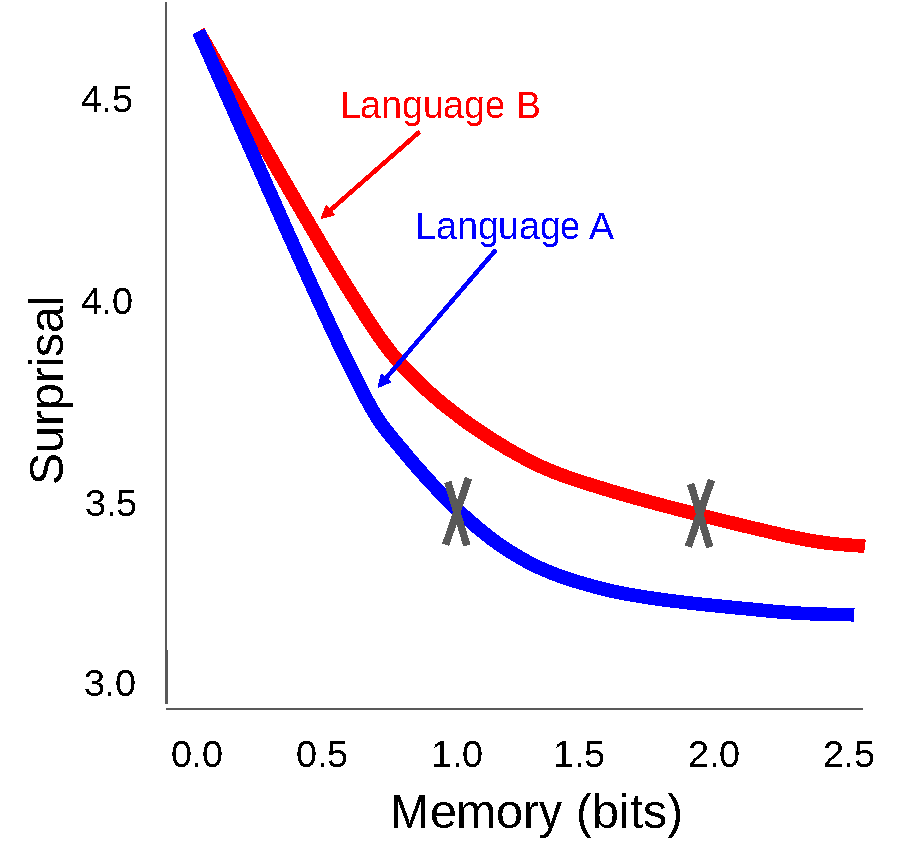
\includegraphics[width=0.5\textwidth]{figures-gdrive/tradeoff-schematic.pdf}
\caption{Example memory--surprisal tradeoff curves for two languages, $A$ and $B$. Achieving an average surprisal of 3.5 bits requires storing at least 1.0 bits in language $A$, while it requires storing 2.0 bits in language $B$. Language $A$ has a steeper memory--surprisal tradeoff than Language $B$, and requires less memory resources to achieve the same level of processing difficulty.}
\label{fig:examples}
\end{figure}

\subsection{Main hypothesis}

Having conceptually introduced the memory--surprisal tradeoff, we can state the main hypothesis of this work, the Efficient Tradeoff Hypothesis.

\begin{adjustwidth}{6em}{6em}
\textbf{Efficient Tradeoff Hypothesis:}\\
The order of elements in natural language is characterized by a distinctively steeper memory--surprisal tradeoff curve, compared to other possible orders.
\end{adjustwidth}
A steep tradeoff curve corresponds to memory efficiency, in the sense that it is possible to achieve a low level of processing difficulty (average surprisal $S_M$) while storing a relatively small amount of information about previous words (entropy of memory $H_M$).
We hypothesize that this property is reflected in grammatical structure and usage preferences across languages.


\subsection{Formal definition of the memory--surprisal tradeoff}
\label{sec:formal-tradeoff}

Here we provide the technical definition of the memory--surprisal tradeoff curve.
Let $W$ be a stochastic process generating a stream of symbols extending indefinitely into the past and future: $\dots, w_{-2}, w_{-1}, w_0, w_{1}, w_{2}, \dots$. %indexed as $w_1, \dots, w_t, \dots$.
These symbols can represent words, morphemes, or other units for decomposing sentences into a sequence of symbols. 
We model this process as stationary \citep{doob1953stochastic}, that is, the joint probability distributions of symbols at different time points depend only on their relative positions in time, not their absolute positions (see SI Section 1.1.1 for more on this modeling assumption).

Let $M$ be a memory encoding function.
We consider memory and surprisal costs at an arbitrary time point $t$.
Recall that the surprisal for a specific word $w_t$ after a past word sequence $\dots, w_{t-2}, w_{t-1}$ encoded into a memory state $m_t$ is:
\begin{equation*}
    -\log P(w_t | m_t).
\end{equation*}
The \key{average surprisal} of the process $W$ under the memory encoding function $M$ is obtained by averaging over all possible past sequences $\dots, w_{t-2}, w_{t-1}$ with associated memory states $m_t$, and possible next words $w_t$:
\begin{equation*}
   S_M \equiv -\sum_{w_t,m_t}  P(m_t) P(w_t|m_t) \log P(w_t | m_t).
\end{equation*}
where $w_t$ ranges over possible symbols, and $m_t$ ranges over possible outputs of the memory encoding function $M$.
This quantity is known as the conditional entropy of $w_t$ given $m_t$ \citep[][p. 17]{cover2006elements}:
\begin{equation*}
	S_M = \operatorname{H}[w_t | m_t].
%    S_M \equiv \lim_{T\rightarrow\infty} \frac{1}{T} \sum_{t=1}^T \operatorname{H}[w_t | m_t],
\end{equation*}
%where the notation $\operatorname{H}[\cdot | \cdot]$ indicates conditional entropy \citep[][p. 17]{cover2006elements}:
%\begin{equation}
%    \operatorname{H}[w_t|m_t] \equiv -\sum_{w_t,m_t} P(m_t) P(w_t|m_t) \log P(w_t|m_t).
%\end{equation}
Because the process $W$ is stationary, the average surprisal $S_M$ is independent of the choice of $t$ (see SI Section 1.1.2).
The lowest possible average surprisal for $W$ is attained when $m_t$ perfectly encodes all previous observed words.
This quantity is called the \key{entropy rate} of $W$ \citep[][pp. 74--75]{cover2006elements}:
\begin{equation*}
    %\label{eq:entropy-rate}
	S_\infty \equiv \operatorname{H}[w_t | \dots, w_{t-2}, w_{t-1}],
%    S_\infty \equiv \lim_{t \rightarrow \infty} \frac{1}{T} \sum_{t=1}^T H[w_t | w_1, \dots, w_{t-1}].
\end{equation*}
which again is independent of $t$ because $W$ is stationary.
We use the notation $S_\infty$ to suggest this idea of unlimited resources.
 The entropy rate of a stochastic process is the irreducible unpredictability of the process: the extent to which a stream of symbols remains unpredictable even for a predictor with unlimited resources. 

 Because the memory state $m_t$ is a function of the previous words $ \dots, w_{t-2}, w_{t-1}$, we can prove by the Data Processing Inequality \citep[][pp. 34--35]{cover2006elements} that the entropy rate must be less than or equal to the average surprisal for any memory encoding function $M$:
\begin{equation*}
    %\label{eq:entropy-rate-dpi}
    S_\infty \le S_M.
\end{equation*}



If the memory state $m_t$ stores all information about the previous words $ \dots, w_{t-2}, w_{t-1}$, then we have $S_M = S_\infty$.
%Based on Eq.~\ref{eq:entropy-rate-dpi}, we can write the average surprisal $S_M$ as a sum of two non-negative terms,
%\begin{equation}
%    S_M = S_\infty + d_M,
%\end{equation}
%where $d_M$ is \key{memory distortion}: the extra surprisal incurred in addition to the unavoidable surprisal $S_\infty$, owing to the lossiness of the memory encoding function $M$. 
%The memory distortion $d_M$ is formally a Kullback-Leibler (KL) divergence:
%\begin{equation}
%    \label{eq:memory-distortion}
%    d_M = \lim_{t \rightarrow \infty} D_{\text{KL}} [ p(w_t | w_1, \dots, w_{t-1}) || p(w_t | m_t)].
%\end{equation}
%Finding a memory encoding function $M$ to minimize $S_M$ is equivalent to minimizing the memory distortion $d_M$.
%\mhahn{do we need to introduce the distortion $d_M$?}

Having defined average surprisal, we now turn to the question of how to define memory capacity. The average amount of information stored in the memory states $m_t$ is the average number of bits required to encode $m_t$. 
This is given by the entropy of the stationary distribution over memory states, $H_M$: %, again averaged over all time points:
\begin{align}
    %\label{eq:memory-entropy}
    \nonumber
        H_M &\equiv \operatorname{H}[m_t] 
    %H_M &\equiv \lim_{T\rightarrow\infty} \frac{1}{T} \sum_{t=1}^T H[m_t] \\
\end{align}
where
\begin{equation*}
    \operatorname{H}[m_t] = - \sum_m P(m_t = m) \log P(m_t=m)
\end{equation*}
where $m$ runs over all possible states of the memory encoding $m_t$.
Again, because $W$ is stationary, this quantity does not depend on the choice of $t$ (see SI Section 1.1.2). 

We will be imposing bounds on $H_M$ and studying the resulting values of $S_M$. 

\begin{definition}
The \key{memory--surprisal tradeoff curve} for a process $W$ is the lowest achievable average surprisal $S_M$ for each value of $H_M$. Let $R$ denote an upper bound on the memory entropy $H_M$; then the memory--surprisal tradeoff curve as a function of $R$ is given by
\begin{equation}
    \label{eq:ms-formal}
    D(R) \equiv \min_{M : H_M \le R} S_M,
\end{equation}
where the minimization is over all memory encoding functions $M$ whose entropy $H_M$ is less than or equal to $R$.
\end{definition}

The memory state $m_t$ is generally a lossy representation of the true context of words $w_1, \dots, w_{t-1}$, meaning that $m_t$ does not contain all the possible information about $w_1, \dots, w_{t-1}$. The mathematical theory of lossy representations is \key{rate--distortion theory} \citep[for an overview and key results, see][pp. 301--347]{cover2006elements}; this theory has seen recent successful application in cognitive science and linguistics as a model of rational action under resource constraints \citep{brady2009compression,sims2012ideal,sims2018efficient,zaslavsky2018efficient,schach2018quantifying,zenon2019information,gershman2020origin}. 
Rate--distortion theory studies curves of the form of Eq.~\ref{eq:ms-formal}, which quantify tradeoffs between negative utility (`distortion') and information (`rate'). %Our memory--surprisal tradeoff curve is a distortion--rate curve, with $H_M$ as the rate and $S_M$ as the distortion. It differs from the typical curve studied in rate--distortion theory in that we define rate using entropy, rather than mutual information \citep[see][for a discussion of some of the consequences of this formulation]{strouse-deterministic-2017}. 
%Our theoretical results still hold if we were to define rate using mutual information (see SI Section \REF).


\begin{figure}
	(a)
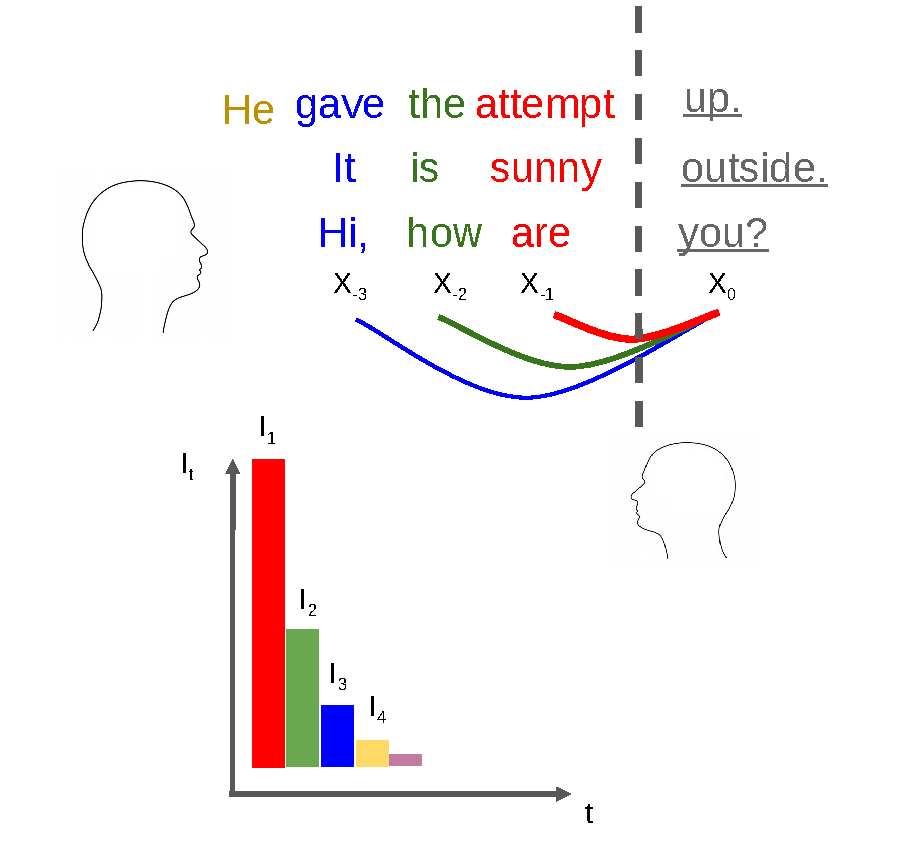
\includegraphics[width=0.4\textwidth]{figures-gdrive/mi-distance.pdf}
	(b)
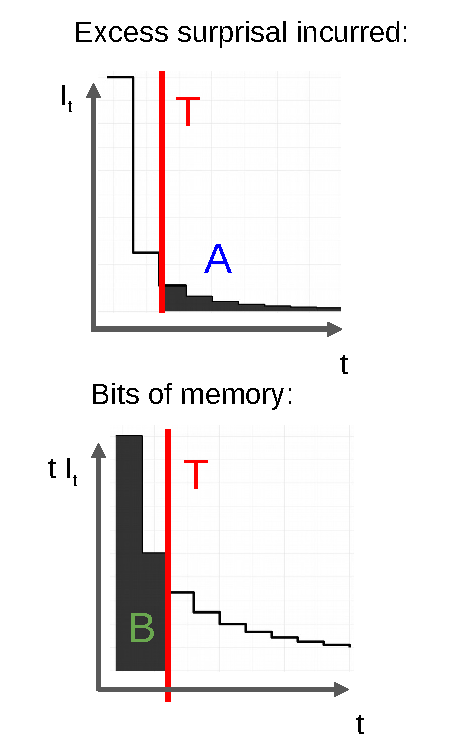
\includegraphics[width=0.25\textwidth]{figures-gdrive/theorem.pdf}
	\caption{
		(a) Conditional mutual information $I_t$ captures how much predictive information about the next word is provided, on average, by the word $t$ steps in the past.
		(b) Here we illustrate our theoretical result. We plot $I_t$ (top) and $tI_t$ (bottom) as functions of $t$. For any choice of $T$, a listener using $B$ bits memory (bottom) to represent prior observations will incur at least $A$ bits of extra surprisal beyond the entropy rate (top). 
}\label{fig:theorem}
\end{figure}

\subsection{Information locality}
\label{sec:infoloc}\label{sec:tradeoff}

The shape of the memory--surprisal tradeoff is determined in part by the grammatical structure of a language.
Some languages enable more efficient tradeoffs than others by allowing a listener to store fewer bits in memory to achieve the same level of average surprisal.

Here, we will demonstrate that the memory--surprisal tradeoff is optimized by languages with word orders exhibiting a property called \key{information locality}. Information locality means that words that depend on each other statistically are located close to each other in time. We will argue that information locality generalizes the well-known word order principle of dependency locality.

We will make our argument by defining a lower bound on the memory--surprisal tradeoff curve (Eq.~\ref{eq:ms-formal}). This lower bound represents an unavoidable cost associated with a certain level of memory usage $H_M$; the true average surprisal $S_M$ might be higher than this bound. 

Our argument will make use of a quantity called \key{mutual information}. Mutual information is the most general measure of statistical association between two random variables. The mutual information between two random variables $X$ and $Y$, conditional on a third random variable $Z$, is defined as:
\begin{align}
\label{eq:mi}
    \operatorname{I}[X:Y|Z] &\equiv \sum_{x,y,z} P(x,y,z) \log \frac{P(x,y|z)}{P(x|z)P(y|z)}. % \text{ bits} \\
    %\nonumber
    %&= \operatorname{H}[X|Z] - \operatorname{H}[X|Y,Z] \\
    %\nonumber
    %&= \operatorname{H}[Y|Z] - \operatorname{H}[Y|X,Z].
\end{align}
Mutual information is always non-negative. It is zero when $X$ and $Y$ are conditionally independent given $Z$, and positive whenever $X$ gives any information that makes the value of $Y$ more predictable, or vice versa. 

We will study the mutual information structure of natural language sentences, and in particular the mutual information between words at certain distances in linear order. We define the notation $I_t$ to mean the mutual information between words at distance $t$ from each other, conditional on the intervening words:
\begin{equation*}
    I_t \equiv \operatorname{I}[w_t : w_0 | w_1, \dots, w_{t-1}].
\end{equation*}
This quantity, visualized in Figure~\ref{fig:theorem}(a), measures how much predictive information is provided about the current word by the word $t$ steps in the past.
It is a statistical property of the language, and can be estimated from large-scale text data.

Equipped with this notion of mutual information at a distance, we can now state our theorem:
\begin{thm}\label{prop:suboptimal}(Information locality bound)
For any positive integer $T$, let $M$ be a memory encoding function such that
\begin{equation}
\label{eq:memory-bound}
H_M \le \sum_{t=1}^T t I_t.    
\end{equation}
Then we have a lower bound on the average surprisal under the memory encoding function $M$:
\begin{equation}
\label{eq:surprisal-bound}
S_M \ge S_\infty + \sum_{t=T+1}^\infty I_t.
\end{equation}
\end{thm}
A formal proof based on the Comprehension Postulates 1--3 is given in SI Section 1.2.
An intuitive argument, forming the basis of the proof, is the following.
Suppose that a comprehender predicting the $t$'th word $w_t$ uses an average of $I_t$ bits of information coming from the previous word $w_0$. 
Then these bits must have been carried over $t$ timesteps and thus have occupied memory for $t$ timesteps.
Since this happens for every word in a sequence, there are, at any given point in time, $t$ such packets of information, each with an average size of $I_t$ bits, that have to be maintained, summing up to $t I_t$.
In the specific setting where $M$ encodes information from a contiguous span of the past $T$ words, the total amount of encoded information thus sums up to $\sum_{t=1}^T t I_t$, while information from longer contexts is lost, increasing surprisal by $\sum_{t=T+1}^\infty I_t$.
While this informal argument specifically considers a memory encoding function that utilizes information from a contiguous span of the past $T$ words, the formal proof extends this to all memory encoding functions $M$ satisfying the Comprehension Postulates.

\paragraph{Interpretation} The theorem means that a predictor with limited memory capacity will always be affected by surprisal cost arising from long-term statistical dependencies of length greater than $T$, for some finite $T$. This is why we call the result `information locality': processes are easier to predict when most statistical dependencies are short-term (shorter than some $T$). Below we explain in more detail how this interpretation matches the mathematics of the theorem.

The quantities in the theorem are illustrated visually in Figure~\ref{fig:theorem}. Eq.~\ref{eq:memory-bound} describes a memory encoding function which has enough capacity to remember the relevant information from at most $T$ words in the immediate past. The minimal amount of memory capacity which would be required to retain this information is the sum $\sum_{t=1}^T t I_t$, reflecting the cost of holding $I_t$ bits in memory for $t$ timesteps up to $t=T$. 

The information locality bound theorem says that the surprisal cost for this memory encoding function is at least $S_\infty + \sum_{t=T+1}^\infty I_t$ (Eq.~\ref{eq:surprisal-bound}). The first term $S_\infty$ is the entropy rate of the process, representing the bits of information in the process which could not have been predicted given any amount of memory. The second term $\sum_{t=T+1}^\infty I_t$ is the sum of all the relevant information contained in words \emph{more} than $T$ timesteps in the past (see Figure~\ref{fig:theorem}(b)). These correspond to bits of information in the process which \emph{could have} been predicted given infinite memory resources, but which were not, due to the limit on memory usage.

The theorem gives a lower bound on the memory--surprisal tradeoff curve, meaning that there is no memory encoding function $M$ with capacity $H_M$ which achieves lower average surprisal than Eq.~\ref{eq:surprisal-bound}. In terms of psycholinguistics, if memory usage is bounded by Eq.~\ref{eq:memory-bound}, then processing cost of at least Eq.~\ref{eq:surprisal-bound} is inevitable.
Importantly, the bound holds for \emph{any} memory encoding function $M$, including functions that do not specifically keep track of a window of the past $T$ words.
The information locality bound theorem demonstrates in a highly general way that language comprehension requires less memory resources when statistical dependencies are mostly short-term. 

\begin{figure*}
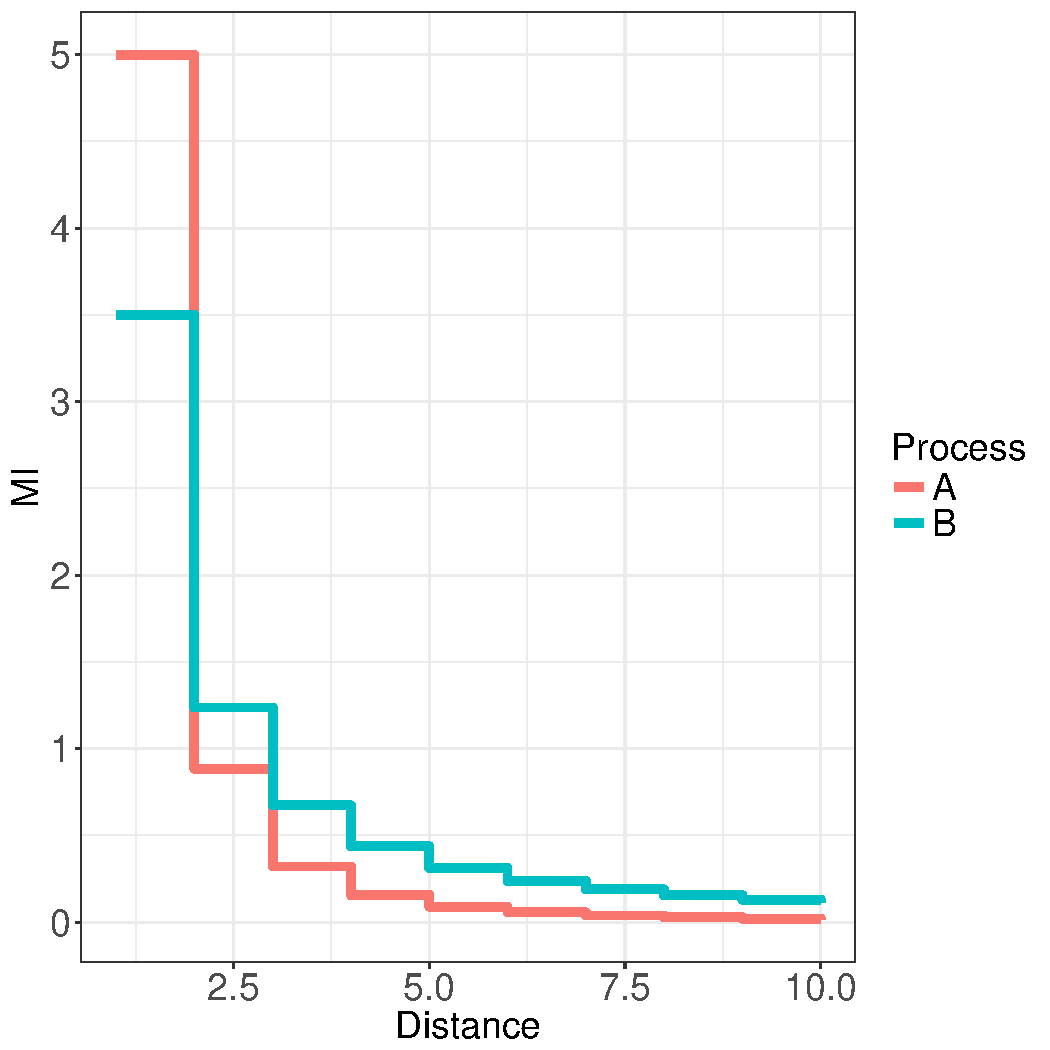
\includegraphics[width=0.45\textwidth]{figures/decay.pdf}
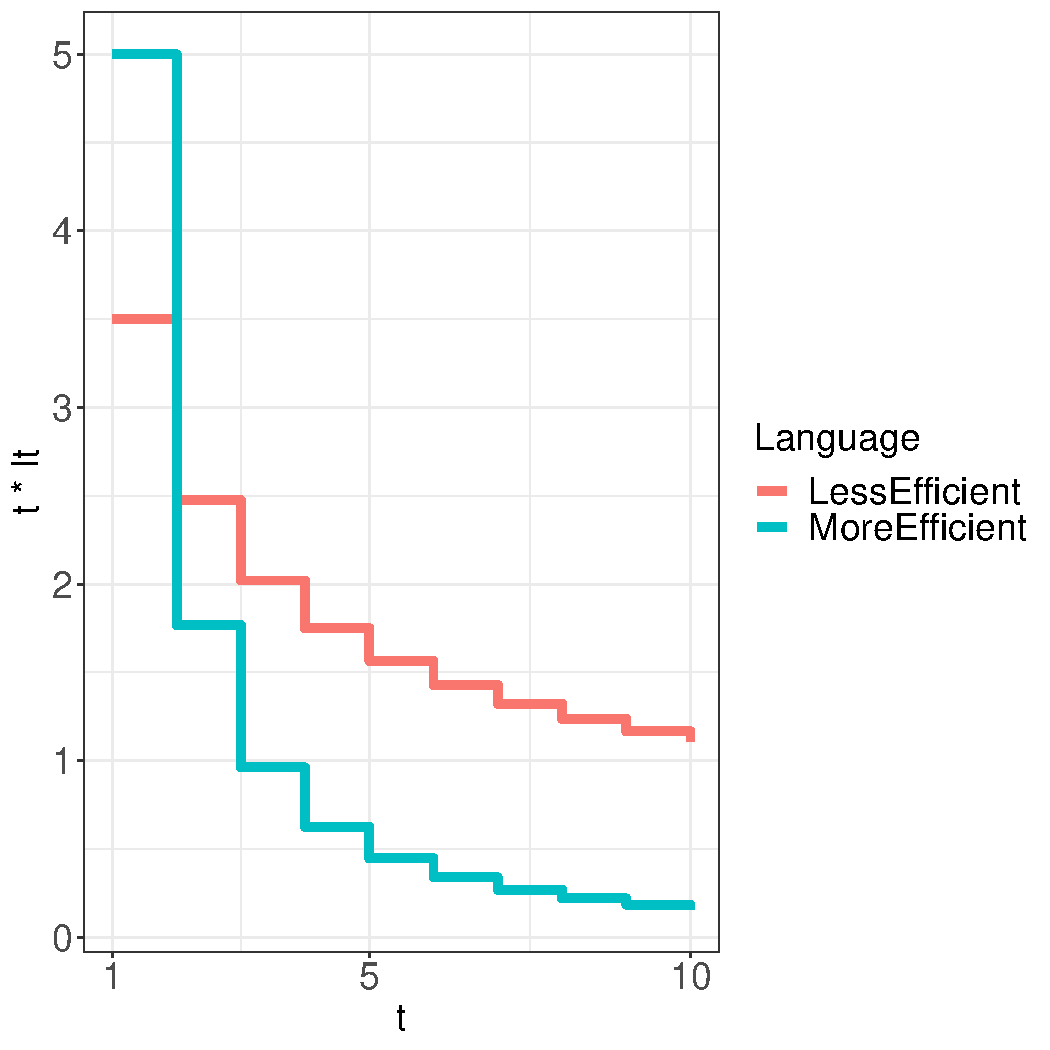
\includegraphics[width=0.45\textwidth]{figures/memory.pdf}
%
	\caption{Left: $I_t$ as a function of $t$, for two different hypothetical languages. $I_t$ decays faster for the MoreEfficient language: Predictive information about the present observation is concentrated more strongly in the recent past. Right: $t \cdot I_t$ as a function of $t$ for the same languages. }\label{fig:basic}
\end{figure*}

\begin{figure}
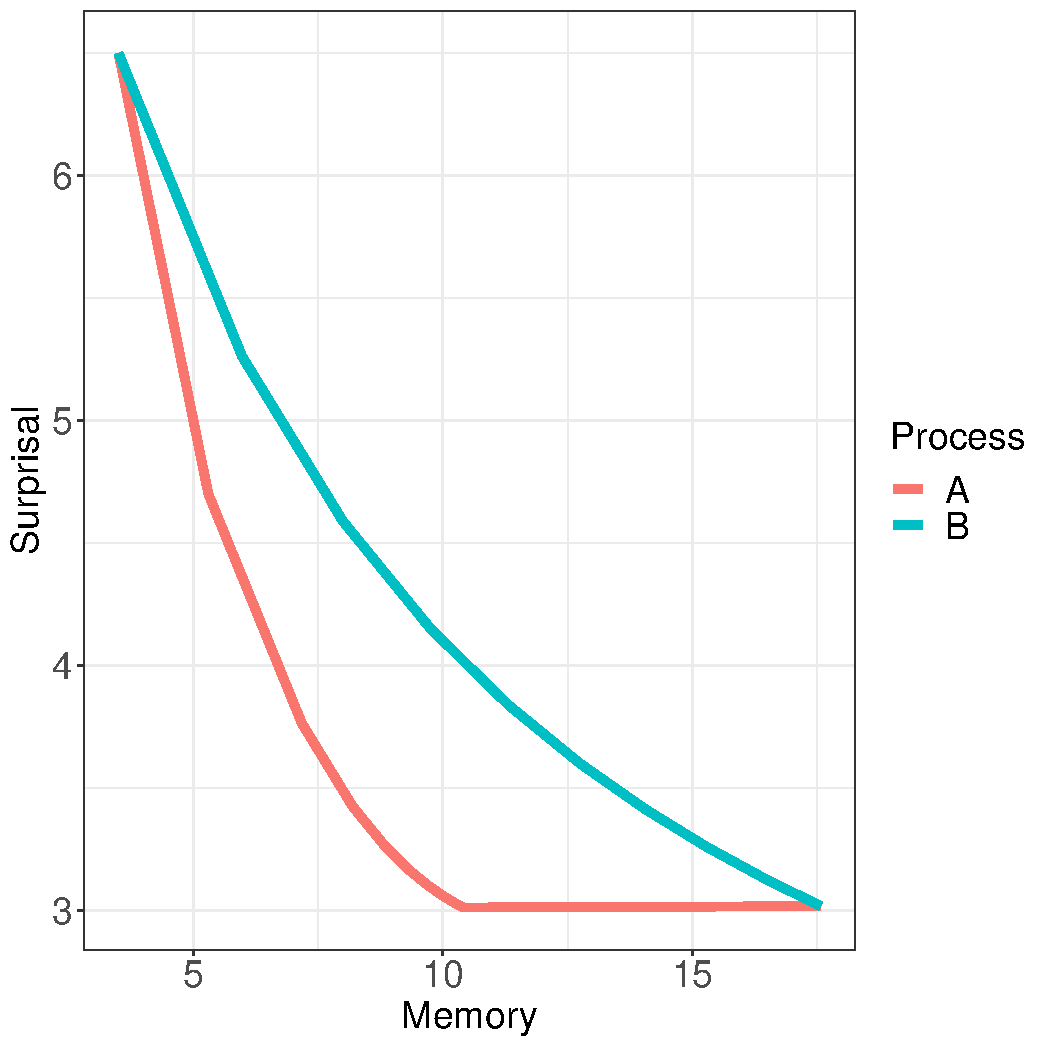
\includegraphics[width=0.45\textwidth]{figures/listener-tradeoff.pdf}
	\caption{Listener's memory--surprisal tradeoff for the two hypothetical languages in Figure~\ref{fig:basic}. Recall that the MoreEfficient language has a faster decay of conditional mutual information $I_t$. Correspondingly, this figure shows that a listener can achieve lower average surprisal at the same level of memory load.}\label{fig:listener-tradeoff}
\end{figure}

%Eq.~\ref{eq:memory-bound} means that maintaining long-term dependencies requires higher memory usage. Carrying the same amount of information over longer distances requires more memory; this fact is reflected in the factor $t$ inside each term of the sum. 
%The result is that modeling long-term statistical dependencies is more costly in terms of memory usage than modeling shorter ones; this cost can manifest in memory storage or in surprisal.


Because processing long-term dependencies requires higher memory usage, the theorem also implies that a language can be easier to process when most of the predictive information about a word is concentrated close to that word in time---that is, when $I_t$ falls off rapidly as $t \rightarrow \infty$. When memory capacity is limited, then there must be some timescale $T$ such that a listener appears to be affected by excess surprisal arising from statistical dependencies of length greater than $T$. A language avoids such cost to the extent that it avoids dependencies with a time-span larger than $T$.

We illustrate the theorem in Figure~\ref{fig:basic}.
We consider two hypothetical languages, LessEfficient and MoreEfficient, where $I_t := 5t^{-1.5}$ for LessEfficient and $I_t := 3.5 t^{-2.5}$ for MoreEfficient.\footnote{Although these are purely mathematical examples, the $I_t$ curve for natural languages does seem empirically to fall off as a power law as in these examples \citep{debowski2016relaxed}.}
The curves of $I_t$, as a function of the distance $t$, are shown in Figure~\ref{fig:basic} (left).
In both cases, $I_t$ converges to zero as $t$ grows to infinity. 
However, $I_t$ decays more quickly for language MoreEfficient.
This means that predictive information about an observation is concentrated more strongly in the recent past.
In Figure~\ref{fig:basic} (right), we show $t\cdot I_t$ as a function of $t$.
Note that the area under the curve is equal to (\ref{eq:memory-bound}).
This area is smaller for the MoreEfficient language, as $I_t$ decays more quickly there.  
In Figure~\ref{fig:listener-tradeoff}, we show the resulting bounds on memory--surprisal tradeoffs of the two languages.  
As $I_t$ decays faster for language MoreEfficient, it has a more efficient memory--surprisal tradeoff, allowing a listener to achieve strictly lower surprisal across a range of memory values.

\subsection{Other kinds of memory bottlenecks}

We derived the memory--surprisal tradeoff and the Information Locality Lower Bound by imposing a capacity limit on memory using the entropy $H_M$. The entropy $H_M$ represents the average amount of information that can be stored in memory at any time. However, in some psycholinguistic theories, memory-related difficulty arises not because of a bound on memory capacity, but rather because of difficulties involved in retrieving information from memory \citep{mcelree2000sentence,lewis-activation-based-2005,nicenboim2018models,vasishth2019computational}. 

It turns out that it is possible to derive results closely analogous to ours by imposing a capacity limit on the retrieval of information from memory, rather than the storage of information. Essentially, the constraint on the memory state in our Theorem~\ref{prop:suboptimal} can be re-interpreted as a constraint on the capacity of a communication channel linking short-term memory to working memory. This result constrains average surprisal for memory models based on cue-based retrieval such as the ACT-R model of \citet{lewis-activation-based-2005}. In fact, the theorem based on retrieval capacity gives a tighter bound than the theorem based on storage capacity. For the full model and derivation, see SI Section 1.3. 

We believe that concepts analogous to the memory--surprisal tradeoff and the Information Locality Lower Bound are likely to be valid across a broad range of models of incremental processing and memory.